\documentclass[9pt]{beamer}

% Beamer style
%\usetheme[secheader]{Madrid}
% \usetheme{CambridgeUS}
\useoutertheme{infolines}
\usecolortheme[rgb={0.65,0.15,0.25}]{structure}
% \usefonttheme[onlymath]{serif}
\beamertemplatenavigationsymbolsempty
%\AtBeginSubsection

% Packags
%\usepackage[french]{babel}
\usepackage[latin1]{inputenc}
\usepackage{color}
\usepackage{xspace}
\usepackage{dsfont, stmaryrd}
\usepackage{amsmath, amsfonts, amssymb}
\usepackage{epsfig}
\usepackage{tikz}
\usepackage{url}
\usepackage{/home/robin/LATEX/Biblio/astats}
%\usepackage[all]{xy}
\usepackage{graphicx}

% Commands
\input{/home/robin/RECHERCHE/EXPOSES/LATEX/Commands}
\definecolor{darkred}{rgb}{0.65,0.15,0.25}
\renewcommand{\newblock}{}

% Tikz
\renewcommand{\nodesize}{1.8em}
\renewcommand{\edgeunit}{2*\nodesize}
\tikzstyle{hidden}=[minimum width=\nodesize, color=gray]
\tikzstyle{observed}=[minimum width=\nodesize]

% Symbols
\newcommand{\Omegas}{\underset{s}{\Omega}}

% Directory
\newcommand{\fignet}{/home/robin/Bureau/RECHERCHE/RESEAUX/EXPOSES/FIGURES}
\newcommand{\figchp}{/home/robin/Bureau/RECHERCHE/RUPTURES/EXPOSES/FIGURES}


%====================================================================
%====================================================================

%====================================================================
%====================================================================
\begin{document}
%====================================================================
%====================================================================

%====================================================================
\title[Joint detection of CNV using coupled HMM]{Joint detection of CNV using coupled HMM}

\author[S. Robin]{\underline{X. Wang}, E. Lebarbier, J. Aubert, S. Robin \\ ~\\}

\institute[INRA/AgroParisTech/Paris-Saclay]{INRA / AgroParisTech /univ. Paris-Saclay \\ ~\\}

\date[Dec. 2018, CNV4Sel]{CNV4Sel, Dec. 2018}

%====================================================================
%====================================================================
\maketitle
%====================================================================

% %====================================================================
% \frame{\frametitle{Outline} \tableofcontents}

%====================================================================
%====================================================================
\section{HMM for CNV detection}
\frame{\frametitle{Outline} \tableofcontents[currentsection]}
%====================================================================
\frame{\frametitle{HMM for CNV detection}

  \paragraph{Data at hand.} SNP array data (for a given chromosome):
  $$
  Y_{it} = \text{signal at position $t$ for individual (line) $i$}
  $$
  
  \bigskip 
  \paragraph{Underlying assumption:} $Y_{it}$ varies according to the copy number at position $t$ \\
  \ra Individual $i$ has a (hidden) 'true' copy number $Z_{it}$ at position $t$.

  \bigskip \bigskip 
  \paragraph{Hidden Markov model.} \refer{CMR05,DEK98}
  \begin{itemize}
   \item $Z_i = (Z_{it})_{1 \leq t \leq T} = $ Markov chain with transition $\pi = (\pi_{k\ell})_{1 \leq k,  \ell \leq K}$
   \item $(Y_{it})_{1 \leq t \leq T}$ independent conditionnally on $Z_i$: $Y_{it} \mid Z_{it} = k \sim F(\theta_k)$
  \end{itemize}
  
  \bigskip 
  \paragraph{In practice:}
  \begin{itemize}
   \item Hidden states. $K = 2:$ \{normal, loss\},  $K = 3:$ \{normal, loss, gain\}
   \item Emission distribution. $F(\theta_k) = \Ncal(\mu_k, \sigma^2)$, $\mu_k \simeq -1, 0, 1$
  \end{itemize}

  }

%====================================================================
\frame{\frametitle{$K = 3$ states: \textcolor{green}{normal}, \textcolor{red}{gain}, \textcolor{black}{loss}}

  $$
  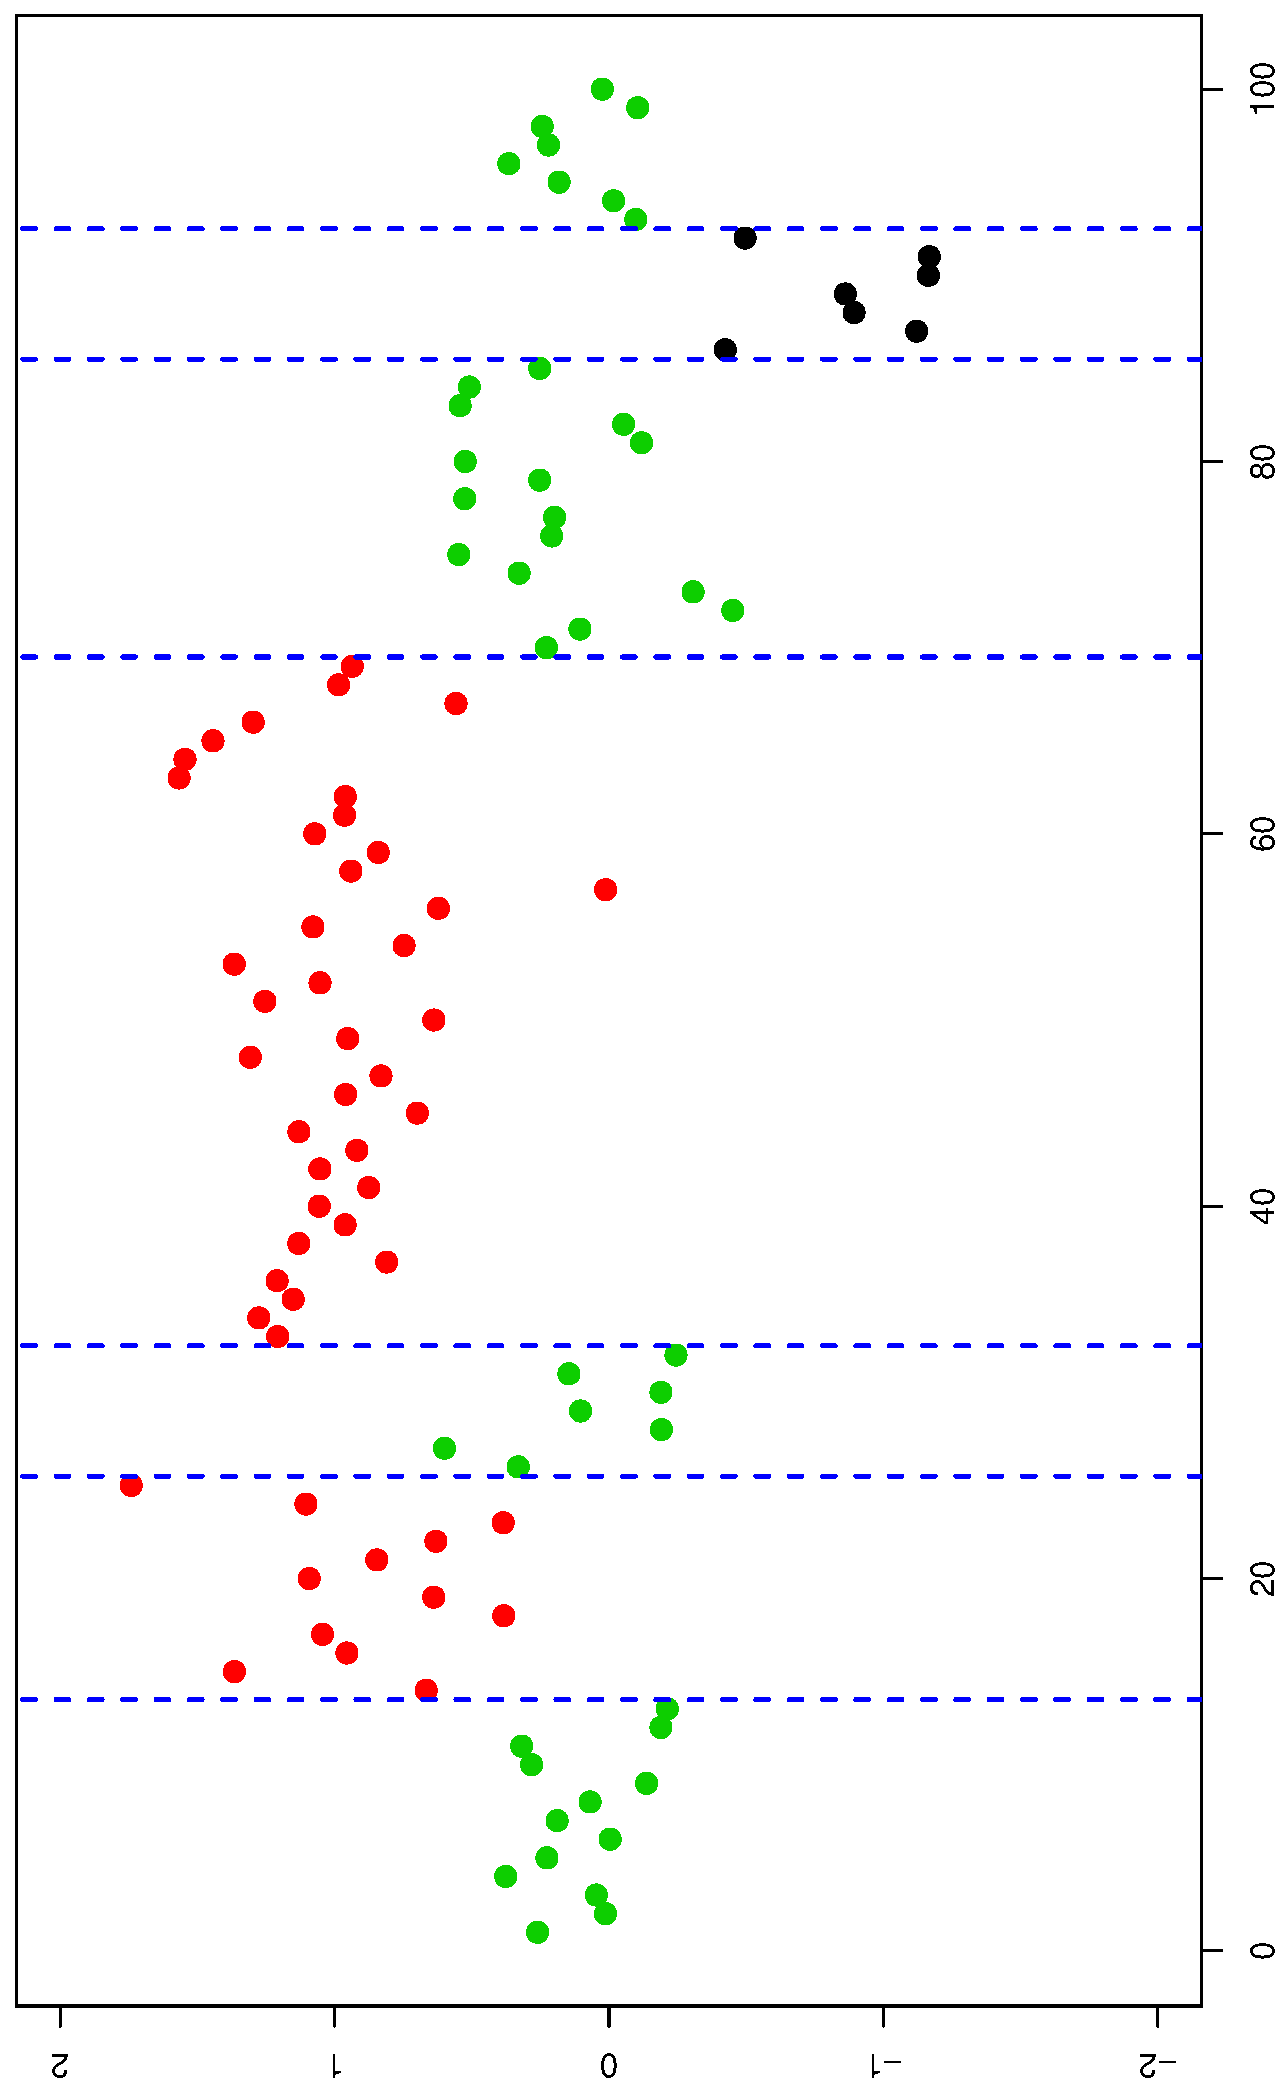
\includegraphics[width=.35\textwidth, angle=270]{../FIGURES/SimHMM_n100_Q3_ZvitXT}   
  $$

  \bigskip \bigskip
  \paragraph{Graphical model.} $Z =$ color, $Y =$ signal
  \begin{center}
%   \includegraphics[scale=.3, clip=true, trim=0 335 65 0]{../Figures/HMModel}
  \begin{tikzpicture}
  \node[hidden] (Z1) at (0, 0) {$Z_{i, 1}$};
  \node[empty] (E1) at (1*\edgeunit, 0) {$\quad$};
  \node[hidden] (Zt) at (2*\edgeunit, 0) {$Z_{i, t}$};
  \node[hidden] (Zt1) at (3*\edgeunit, 0) {$Z_{i, t+1}$};
  \node[empty] (Et1) at (4*\edgeunit, 0) {$\quad$};
  \node[hidden] (ZT) at (5*\edgeunit, 0) {$Z_{i, T}$};

  \node[observed] (Y1) at (0.25, -1*\edgeunit) {$Y_{i, 1}$};
  \node[observed] (Yt) at (2.25*\edgeunit, -1*\edgeunit) {$Y_{i, t}$};
  \node[observed] (Yt1) at (3.25*\edgeunit, -1*\edgeunit) {$Y_{i, t+1}$};
  \node[observed] (YT) at (5.25*\edgeunit, -1*\edgeunit) {$Y_{i, T}$};

  \draw[lightarrow] (Z1) to (E1);
  \draw[lightarrow] (E1) to (Zt);
  \draw[lightarrow] (Zt) to (Zt1);
  \draw[lightarrow] (Zt1) to (Et1);
  \draw[lightarrow] (Et1) to (ZT);

  \draw[arrow] (Z1) to (Y1);
  \draw[arrow] (Zt) to (Yt);
  \draw[arrow] (Zt1) to (Yt1);
  \draw[arrow] (ZT) to (YT);

  \end{tikzpicture}
  \end{center}


}
  

%====================================================================
\frame{\frametitle{Inference}

  \paragraph{Graphical model:}
  \begin{center}
%   \includegraphics[scale=.3, clip=true, trim=0 335 65 0]{../Figures/HMModel}
  \begin{tikzpicture}
  \node[hidden] (Z1) at (0, 0) {$Z_{i, 1}$};
  \node[empty] (E1) at (1*\edgeunit, 0) {$\quad$};
  \node[hidden] (Zt) at (2*\edgeunit, 0) {$Z_{i, t}$};
  \node[hidden] (Zt1) at (3*\edgeunit, 0) {$Z_{i, t+1}$};
  \node[empty] (Et1) at (4*\edgeunit, 0) {$\quad$};
  \node[hidden] (ZT) at (5*\edgeunit, 0) {$Z_{i, T}$};

  \node[observed] (Y1) at (0.25, -1*\edgeunit) {$Y_{i, 1}$};
  \node[observed] (Yt) at (2.25*\edgeunit, -1*\edgeunit) {$Y_{i, t}$};
  \node[observed] (Yt1) at (3.25*\edgeunit, -1*\edgeunit) {$Y_{i, t+1}$};
  \node[observed] (YT) at (5.25*\edgeunit, -1*\edgeunit) {$Y_{i, T}$};

  \draw[lightarrow] (Z1) to (E1);
  \draw[lightarrow] (E1) to (Zt);
  \draw[lightarrow] (Zt) to (Zt1);
  \draw[lightarrow] (Zt1) to (Et1);
  \draw[lightarrow] (Et1) to (ZT);

  \draw[arrow] (Z1) to (Y1);
  \draw[arrow] (Zt) to (Yt);
  \draw[arrow] (Zt1) to (Yt1);
  \draw[arrow] (ZT) to (YT);

  \end{tikzpicture}
  \end{center}
  
  \bigskip
  \paragraph{EM algorithm:}
  \begin{itemize}
  \item E step: 'retrieve' the hidden states: $P(Z_{it} = k \mid Y_i)$ \\
  \ra Forward-backward recursion: complexity $= \emphase{O(T K^2)}$
  \item M step: update the estimates $\widehat{\mu}_k$,  $\widehat{\sigma}^2$, $\widehat{\pi}_{k\ell}$
  \end{itemize}
  
  \bigskip \bigskip
  \paragraph{'Calling':}
  \begin{itemize}
  \item Position by position, according to $P(Z_{it} = k \mid Y_i)$
  \item Whole path: most probable sequence $Z_i$ given $Y_i$ (Viterbi algorithm: $\emphase{O(T K^2)}$) 
  \end{itemize}
  }


%====================================================================
\frame{\frametitle{HMM for several profiles}

  \paragraph{Graphical model:}
  \begin{center}
%   \includegraphics[scale=.3, clip=true, trim=0 335 65 0]{../Figures/HMModel}
  \begin{tikzpicture}
  % Profile 1
  \node[hidden] (Z11) at (0, 0) {$Z_{1, 1}$};
  \node[empty] (E11) at (1*\edgeunit, 0) {$\quad$};
  \node[hidden] (Z1t) at (2*\edgeunit, 0) {$Z_{1, t}$};
  \node[hidden] (Z1t1) at (3*\edgeunit, 0) {$Z_{1, t+1}$};
  \node[empty] (E1t1) at (4*\edgeunit, 0) {$\quad$};
  \node[hidden] (Z1T) at (5*\edgeunit, 0) {$Z_{1, T}$};

  \node[observed] (Y11) at (.5, -.75*\edgeunit) {$Y_{1, 1}$};
  \node[observed] (Y1t) at (2.5*\edgeunit, -.75*\edgeunit) {$Y_{1, t}$};
  \node[observed] (Y1t1) at (3.5*\edgeunit, -.75*\edgeunit) {$Y_{1, t+1}$};
  \node[observed] (Y1T) at (5.5*\edgeunit, -.75*\edgeunit) {$Y_{1, T}$};

  \draw[lightarrow] (Z11) to (E11); \draw[lightarrow] (E11) to (Z1t);
  \draw[lightarrow] (Z1t) to (Z1t1); \draw[lightarrow] (Z1t1) to (E1t1);
  \draw[lightarrow] (E1t1) to (Z1T);

  \draw[arrow] (Z11) to (Y11); \draw[arrow] (Z1t) to (Y1t);
  \draw[arrow] (Z1t1) to (Y1t1); \draw[arrow] (Z1T) to (Y1T);

  % Profile 2
  \node[hidden] (Z21) at (0, -1.5) {$Z_{2,1}$};
  \node[empty] (E21) at (1*\edgeunit, -1.5) {$\quad$};
  \node[hidden] (Z2t) at (2*\edgeunit, -1.5) {$Z_{2,t}$};
  \node[hidden] (Z2t1) at (3*\edgeunit, -1.5) {$Z_{2,t+1}$};
  \node[empty] (E2t1) at (4*\edgeunit, -1.5) {$\quad$};
  \node[hidden] (Z2T) at (5*\edgeunit, -1.5) {$Z_{2,T}$};

  \node[observed] (Y21) at (.5, -2*\edgeunit) {$Y_{2,1}$};
  \node[observed] (Y2t) at (2.5*\edgeunit, -2*\edgeunit) {$Y_{2,t}$};
  \node[observed] (Y2t1) at (3.5*\edgeunit, -2*\edgeunit) {$Y_{2,t+1}$};
  \node[observed] (Y2T) at (5.5*\edgeunit, -2*\edgeunit) {$Y_{2,T}$};

  \draw[lightarrow] (Z21) to (E21); \draw[lightarrow] (E21) to (Z2t);
  \draw[lightarrow] (Z2t) to (Z2t1); \draw[lightarrow] (Z2t1) to (E2t1);
  \draw[lightarrow] (E2t1) to (Z2T);

  \draw[arrow] (Z21) to (Y21); \draw[arrow] (Z2t) to (Y2t);
  \draw[arrow] (Z2t1) to (Y2t1); \draw[arrow] (Z2T) to (Y2T);
  
  % Profile 3
  \node[hidden] (Z31) at (0, -3) {$Z_{3,1}$};
  \node[empty] (E31) at (1*\edgeunit, -3) {$\quad$};
  \node[hidden] (Z3t) at (2*\edgeunit, -3) {$Z_{3,t}$};
  \node[hidden] (Z3t1) at (3*\edgeunit, -3) {$Z_{3,t+1}$};
  \node[empty] (E3t1) at (4*\edgeunit, -3) {$\quad$};
  \node[hidden] (Z3T) at (5*\edgeunit, -3) {$Z_{3,T}$};

  \node[observed] (Y31) at (.5, -3.3*\edgeunit) {$Y_{3,1}$};
  \node[observed] (Y3t) at (2.5*\edgeunit, -3.3*\edgeunit) {$Y_{3,t}$};
  \node[observed] (Y3t1) at (3.5*\edgeunit, -3.3*\edgeunit) {$Y_{3,t+1}$};
  \node[observed] (Y3T) at (5.5*\edgeunit, -3.3*\edgeunit) {$Y_{3,T}$};

  \draw[lightarrow] (Z31) to (E31); \draw[lightarrow] (E31) to (Z3t);
  \draw[lightarrow] (Z3t) to (Z3t1); \draw[lightarrow] (Z3t1) to (E3t1);
  \draw[lightarrow] (E3t1) to (Z3T);

  \draw[arrow] (Z31) to (Y31); \draw[arrow] (Z3t) to (Y3t);
  \draw[arrow] (Z3t1) to (Y3t1); \draw[arrow] (Z3T) to (Y3T);
  
  \end{tikzpicture}
  \end{center}
  
  \bigskip
  \paragraph{Inference} $\simeq I$ independent HMM: $\emphase{O(I T K^2)}$
  }

%====================================================================
%====================================================================
\section{Accounting for similarity between lines}
\frame{\frametitle{Outline} \tableofcontents[currentsection]}
%====================================================================
\frame{\frametitle{Accounting for genetic similarity}

  \paragraph{Additional information.} $S = (s_{ij})_{1 \leq i, j \leq I}$
  $$
  s_{ij} = \text{similarity between individuals $i$ and $j$}
  $$
  e.g. $S = $ kinship matrix.
  
  \bigskip \bigskip 
  \paragraph{Rational.} At any given position $t$, two individuals $i$ and $j$ with high similarity are likely to share the same hidden state $Z_{it}$ and $Z_{jt}$
  $$
  P(Z_{it} = \ell \mid Z_{i,t-1} = k, (Z_{jt})_{j \neq i}) 
  \; \propto \;
  \emphase{\pi_{k\ell}} \prod_{j \neq i} w^{s_{ij} \Ibb\{\ell_j \neq \ell\}}, 
  \qquad 
  0 \leq \emphase{w} \leq 1
  $$
  \ra The hidden states are not independent from one individual to another
  }
  
%====================================================================
\frame{\frametitle{Coupled HMM}

  \paragraph{Graphical model.} \refer{Mur02}
  \begin{center}
%   \includegraphics[scale=.3, clip=true, trim=0 335 65 0]{../Figures/HMModel}
  \begin{tikzpicture}
  % Profile 1
  \node[hidden] (Z11) at (0, 0) {$Z_{1, 1}$};
  \node[empty] (E11) at (1*\edgeunit, 0) {$\quad$};
  \node[hidden] (Z1t) at (2*\edgeunit, 0) {$Z_{1, t}$};
  \node[hidden] (Z1t1) at (3*\edgeunit, 0) {$Z_{1, t+1}$};
  \node[empty] (E1t1) at (4*\edgeunit, 0) {$\quad$};
  \node[hidden] (Z1T) at (5*\edgeunit, 0) {$Z_{1, T}$};

  \node[observed] (Y11) at (.5, -.75*\edgeunit) {$Y_{1, 1}$};
  \node[observed] (Y1t) at (2.5*\edgeunit, -.75*\edgeunit) {$Y_{1, t}$};
  \node[observed] (Y1t1) at (3.5*\edgeunit, -.75*\edgeunit) {$Y_{1, t+1}$};
  \node[observed] (Y1T) at (5.5*\edgeunit, -.75*\edgeunit) {$Y_{1, T}$};

  \draw[lightarrow] (Z11) to (E11); \draw[lightarrow] (E11) to (Z1t);
  \draw[lightarrow] (Z1t) to (Z1t1); \draw[lightarrow] (Z1t1) to (E1t1);
  \draw[lightarrow] (E1t1) to (Z1T);

  \draw[arrow] (Z11) to (Y11); \draw[arrow] (Z1t) to (Y1t);
  \draw[arrow] (Z1t1) to (Y1t1); \draw[arrow] (Z1T) to (Y1T);

  % Profile 2
  \node[hidden] (Z21) at (0, -1.5) {$Z_{2,1}$};
  \node[empty] (E21) at (1*\edgeunit, -1.5) {$\quad$};
  \node[hidden] (Z2t) at (2*\edgeunit, -1.5) {$Z_{2,t}$};
  \node[hidden] (Z2t1) at (3*\edgeunit, -1.5) {$Z_{2,t+1}$};
  \node[empty] (E2t1) at (4*\edgeunit, -1.5) {$\quad$};
  \node[hidden] (Z2T) at (5*\edgeunit, -1.5) {$Z_{2,T}$};

  \node[observed] (Y21) at (.5, -2*\edgeunit) {$Y_{2,1}$};
  \node[observed] (Y2t) at (2.5*\edgeunit, -2*\edgeunit) {$Y_{2,t}$};
  \node[observed] (Y2t1) at (3.5*\edgeunit, -2*\edgeunit) {$Y_{2,t+1}$};
  \node[observed] (Y2T) at (5.5*\edgeunit, -2*\edgeunit) {$Y_{2,T}$};

  \draw[lightarrow] (Z21) to (E21); \draw[lightarrow] (E21) to (Z2t);
  \draw[lightarrow] (Z2t) to (Z2t1); \draw[lightarrow] (Z2t1) to (E2t1);
  \draw[lightarrow] (E2t1) to (Z2T);

  \draw[arrow] (Z21) to (Y21); \draw[arrow] (Z2t) to (Y2t);
  \draw[arrow] (Z2t1) to (Y2t1); \draw[arrow] (Z2T) to (Y2T);
  
  % Profile 3
  \node[hidden] (Z31) at (0, -3) {$Z_{3,1}$};
  \node[empty] (E31) at (1*\edgeunit, -3) {$\quad$};
  \node[hidden] (Z3t) at (2*\edgeunit, -3) {$Z_{3,t}$};
  \node[hidden] (Z3t1) at (3*\edgeunit, -3) {$Z_{3,t+1}$};
  \node[empty] (E3t1) at (4*\edgeunit, -3) {$\quad$};
  \node[hidden] (Z3T) at (5*\edgeunit, -3) {$Z_{3,T}$};

  \node[observed] (Y31) at (.5, -3.3*\edgeunit) {$Y_{3,1}$};
  \node[observed] (Y3t) at (2.5*\edgeunit, -3.3*\edgeunit) {$Y_{3,t}$};
  \node[observed] (Y3t1) at (3.5*\edgeunit, -3.3*\edgeunit) {$Y_{3,t+1}$};
  \node[observed] (Y3T) at (5.5*\edgeunit, -3.3*\edgeunit) {$Y_{3,T}$};

  \draw[lightarrow] (Z31) to (E31); \draw[lightarrow] (E31) to (Z3t);
  \draw[lightarrow] (Z3t) to (Z3t1); \draw[lightarrow] (Z3t1) to (E3t1);
  \draw[lightarrow] (E3t1) to (Z3T);

  \draw[arrow] (Z31) to (Y31); \draw[arrow] (Z3t) to (Y3t);
  \draw[arrow] (Z3t1) to (Y3t1); \draw[arrow] (Z3T) to (Y3T);
  
  % Between profiles
  \draw[lightedge] (Z11) to (Z21); \draw[lightedge] (Z11) to [bend right](Z31); \draw[lightedge] (Z21) to (Z31);  
  \draw[lightedge] (Z1t) to (Z2t); \draw[lightedge] (Z1t) to [bend right](Z3t); \draw[lightedge] (Z2t) to (Z3t);  
  \draw[lightedge] (Z1t1) to (Z2t1); \draw[lightedge] (Z1t1) to [bend right](Z3t1); \draw[lightedge] (Z2t1) to (Z3t1);  
  \draw[lightedge] (Z1T) to (Z2T); \draw[lightedge] (Z1T) to [bend right](Z3T); \draw[lightedge] (Z2T) to (Z3T);  
  \end{tikzpicture}
  \end{center}
  
  \paragraph{Inference.} 
  \begin{itemize}
   \item Naive point of view: one 'big' HMM with $K^I$ hidden states: $\emphase{O(T K^{2I})}$
   \item \emphase{Variational approximation} \refer{WaJ08} of $P((Z_{it})_{1 \leq i \leq I} \mid Y)$: back to $\emphase{O(\max(I T K^2, T I^2)}$ 
   \item Paper \refer{WLA18} + R package {\tt CHMM}
  \end{itemize}
  
  }


%====================================================================
%====================================================================
\section{Illustrations}
\frame{\frametitle{Outline} \tableofcontents[currentsection]}
%====================================================================
\frame{\frametitle{Simulations}

  \paragraph{Running time (s).} $T = 1000$, $K=3$, $K^2 = 9$
  \begin{center}
  \begin{tabular}{c|ccc|c}
  $I$ & {indep. EM} & \emphase{coupled VEM} & coupled EM  & $K^{2I}$ \\ 
  \hline
  2 & 0.8 & 0.4 & 2.0 & 81 \\ 
  3 & 1.1 & 0.5 & 11.2 & 729 \\ 
  4 & 1.2 & 0.6 & 79.4 & 6561 \\ 
  5 & 1.6 & 0.8 & 920.2 & 59049 \\ 
  \end{tabular}
  \end{center}
  ($I = 10, K ^{2I} \simeq 3 \; 10^9$)
  
  \bigskip \bigskip 
  \paragraph{Accuracy.} $T = 1000$, $I = 3$ individuals, $K = 3$ states: $\mu_k = -1, 0, 1$
  $$
  \begin{array}{c}
  \sigma = 0.3 \hspace{.15\textwidth} \sigma = 1 \hspace{.15\textwidth} \sigma = 1.2 \\
  \includegraphics[height=.3\textheight, width=.7\textwidth]{../FIGURES/WLA18-Fig3.pdf} \\
  \text{iHMM-EM / cHMM-VEM / cHMM-EM}
  \end{array}
  $$

  }

%====================================================================
\frame{\frametitle{Sheep data (T. Faraut, J. Aubert)}

  \paragraph{Data.} $I = 26$ individuals, 1 chromosome, $T = 62210$ probes, $\simeq$ every 5kb

  \bigskip 
  \paragraph{Results.} $K = 5$ states: $\widehat{\sigma} = .12$, 
  $$
  \begin{array}{crrrrr}
   \text{state} & 1 & 2 & 3 & 4 & 5 \\
   \hline
   \widehat{\mu}_k & -0.86 & -0.44 & -0.15 & -0.01  & 0.08 \\
   N_k & 3960 & 31906 & 603 & 34736 & 40
  \end{array}
  $$
  including 9 individuals with a long deletion ($>$ 27 kb)
  
  \bigskip
  \paragraph{Clustering.} 
  $$
  \includegraphics[width=.5\textwidth]{CNV_TFaraut_cluster}
  $$
  

  }

%====================================================================
\frame[allowframebreaks]{ \frametitle{References}
{\tiny
  \bibliography{/home/robin/Biblio/BibGene}
%   \bibliographystyle{/home/robin/LATEX/Biblio/astats}
  \bibliographystyle{alpha}
  }
}

%====================================================================
\backupbegin

%====================================================================
\backupend

%====================================================================
%====================================================================
\end{document}
%====================================================================
%====================================================================

  \begin{tabular}{cc}
    \begin{tabular}{p{.5\textwidth}}
    \end{tabular}
    & 
    \hspace{-.02\textwidth}
    \begin{tabular}{p{.5\textwidth}}
    \end{tabular}
  \end{tabular}

